
\documentclass[letter]{moderncv} % Font sizes: 10, 11, or 12; paper sizes: a4paper, letterpaper, a5paper, legalpaper, executivepaper or landscape; font families: sans or roman
\usepackage[margin=30pt]{geometry}
\moderncvstyle{classic} % CV theme - options include: 'casual' (default), 'classic', 'oldstyle' and 'banking'
\moderncvcolor{blue} % CV color - options include: 'blue' (default), 'orange', 'green', 'red', 'purple', 'grey' and 'black'


%\setlength{\hintscolumnwidth}{3cm} % Uncomment to change the width of the dates column
%\setlength{\makecvtitlenamewidth}{10cm} % For the 'classic' style, uncomment to adjust the width of the space allocated to your name

%----------------------------------------------------------------------------------------
%	NAME AND CONTACT INFORMATION SECTION
%----------------------------------------------------------------------------------------

\firstname{} % Title is Misused here
\familyname{}
\title{\textbf{\textcolor{black}{IEEE CTW 2019 -- Positioning Competition}}} %Deutsch
%----------------------------------------------------------------------------------------

\begin{document}

\includegraphics[width=1\textwidth]{Comsoc}
\maketitle % Print the CV title
\vspace{-4ex}
\section{Background}
Due to the huge success of mobile communications in almost any area of modern life, indoor positioning systems   receive large attention from both industry and academia. 
Indoor positioning  is  a key enabler for a wide range of applications such as indoor navigation, smart factories, surveillance, security, smart cities, IoT, and sensor networks. 
Additionally, indoor positioning  can be leveraged for improved beamforming and  channel estimation in wireless communications. 

%Given the impact of IPS, this CTW competition presents a dataset of channel state information obtained for a massive multiple-input multiple-output (MIMO)-orthogonal frequency division multiplex (OFDM) channel sounder [1], for indoor positioning. 


%\bigskip

%\textcolor{red}{If you are allowed to deviate from the original text, one could do as below:}

%\textcolor{red}{Given the rise of machine learning and the abundant amount of data available by wireless systems, user positioning based on wireless systems is receiving significant attention from academia and industry.  User poisoning systems are a key enabler for many applications and concepts like navigation systems, smart cities, security and surveillance, internet of things, etc. Therefore, this CTW competition presents a dataset of channel state information obtained for a massive multiple-input multiple-output (MIMO) channel sounder for indoor positioning [1], hoping that cultivates further algorithmic innovations in this context.}

\section{The Competition and Evaluation Criteria}

The task is to estimate a user position based on frequency responses of a channel between a user at an unknown location and an array of antennas. 
Possible solutions may include classic approaches (fingerprinting, interpolation) as well as deep-learning based approaches. 
Channel vectors from  the dataset created with the channel sounder in [1] will be used.

~

To compete, teams may download the dataset and develop algorithms. The dataset contains i) channel responses, ii) ground truth positions, and iii) SNR information. (See below for more detail.)
The dataset may be partitioned into training and test sets as found appropriate for
the algorithm training and development.

~

In the morning of May 26.5.2019, at IEEE CTW, a set of test data will be distributed. Participating teams may run their algorithms on this test data set, and submit their
estimated position coordinates to  \\
\texttt{data-competition@inue.uni-stuttgart.de} no later than 20:00.
Winners will be determined by the organizers by evaluating and comparing the root-mean-square position error. (Ground truth will not be available to the
participants, and the test dataset will not be available before the conference. It will be averaged over all test positions)

~

A prize will be given to the best three competing teams.

%Each individual person or team is allowed to submit (up to three) solutions (prediction on the h\_Estimated\_Test.mat) to and present their solution on the CTW as a poster. A prize will be given out for the first three candidates.
%The metric for evalation is $\mathrm{E}(|d-\hat{d}|)$, with $\hat{d}$ being the estimated user position.

\section{About the Dataset}

A massive MIMO channel sounder was used to acquire channel responses between a transmitter and an 8$\times$2 antenna array [1]. An SDR-equipped vacuum-cleaner robot drove in a random path on a ~4$\times$2m table and transmitted uplink OFDM pilots with a bandwidth of 20~MHz and 1024 subcarriers at a carrier frequency of 1.25GHz. 10 \% of the subcarriers were used as guard bands.
\vspace{2ex}

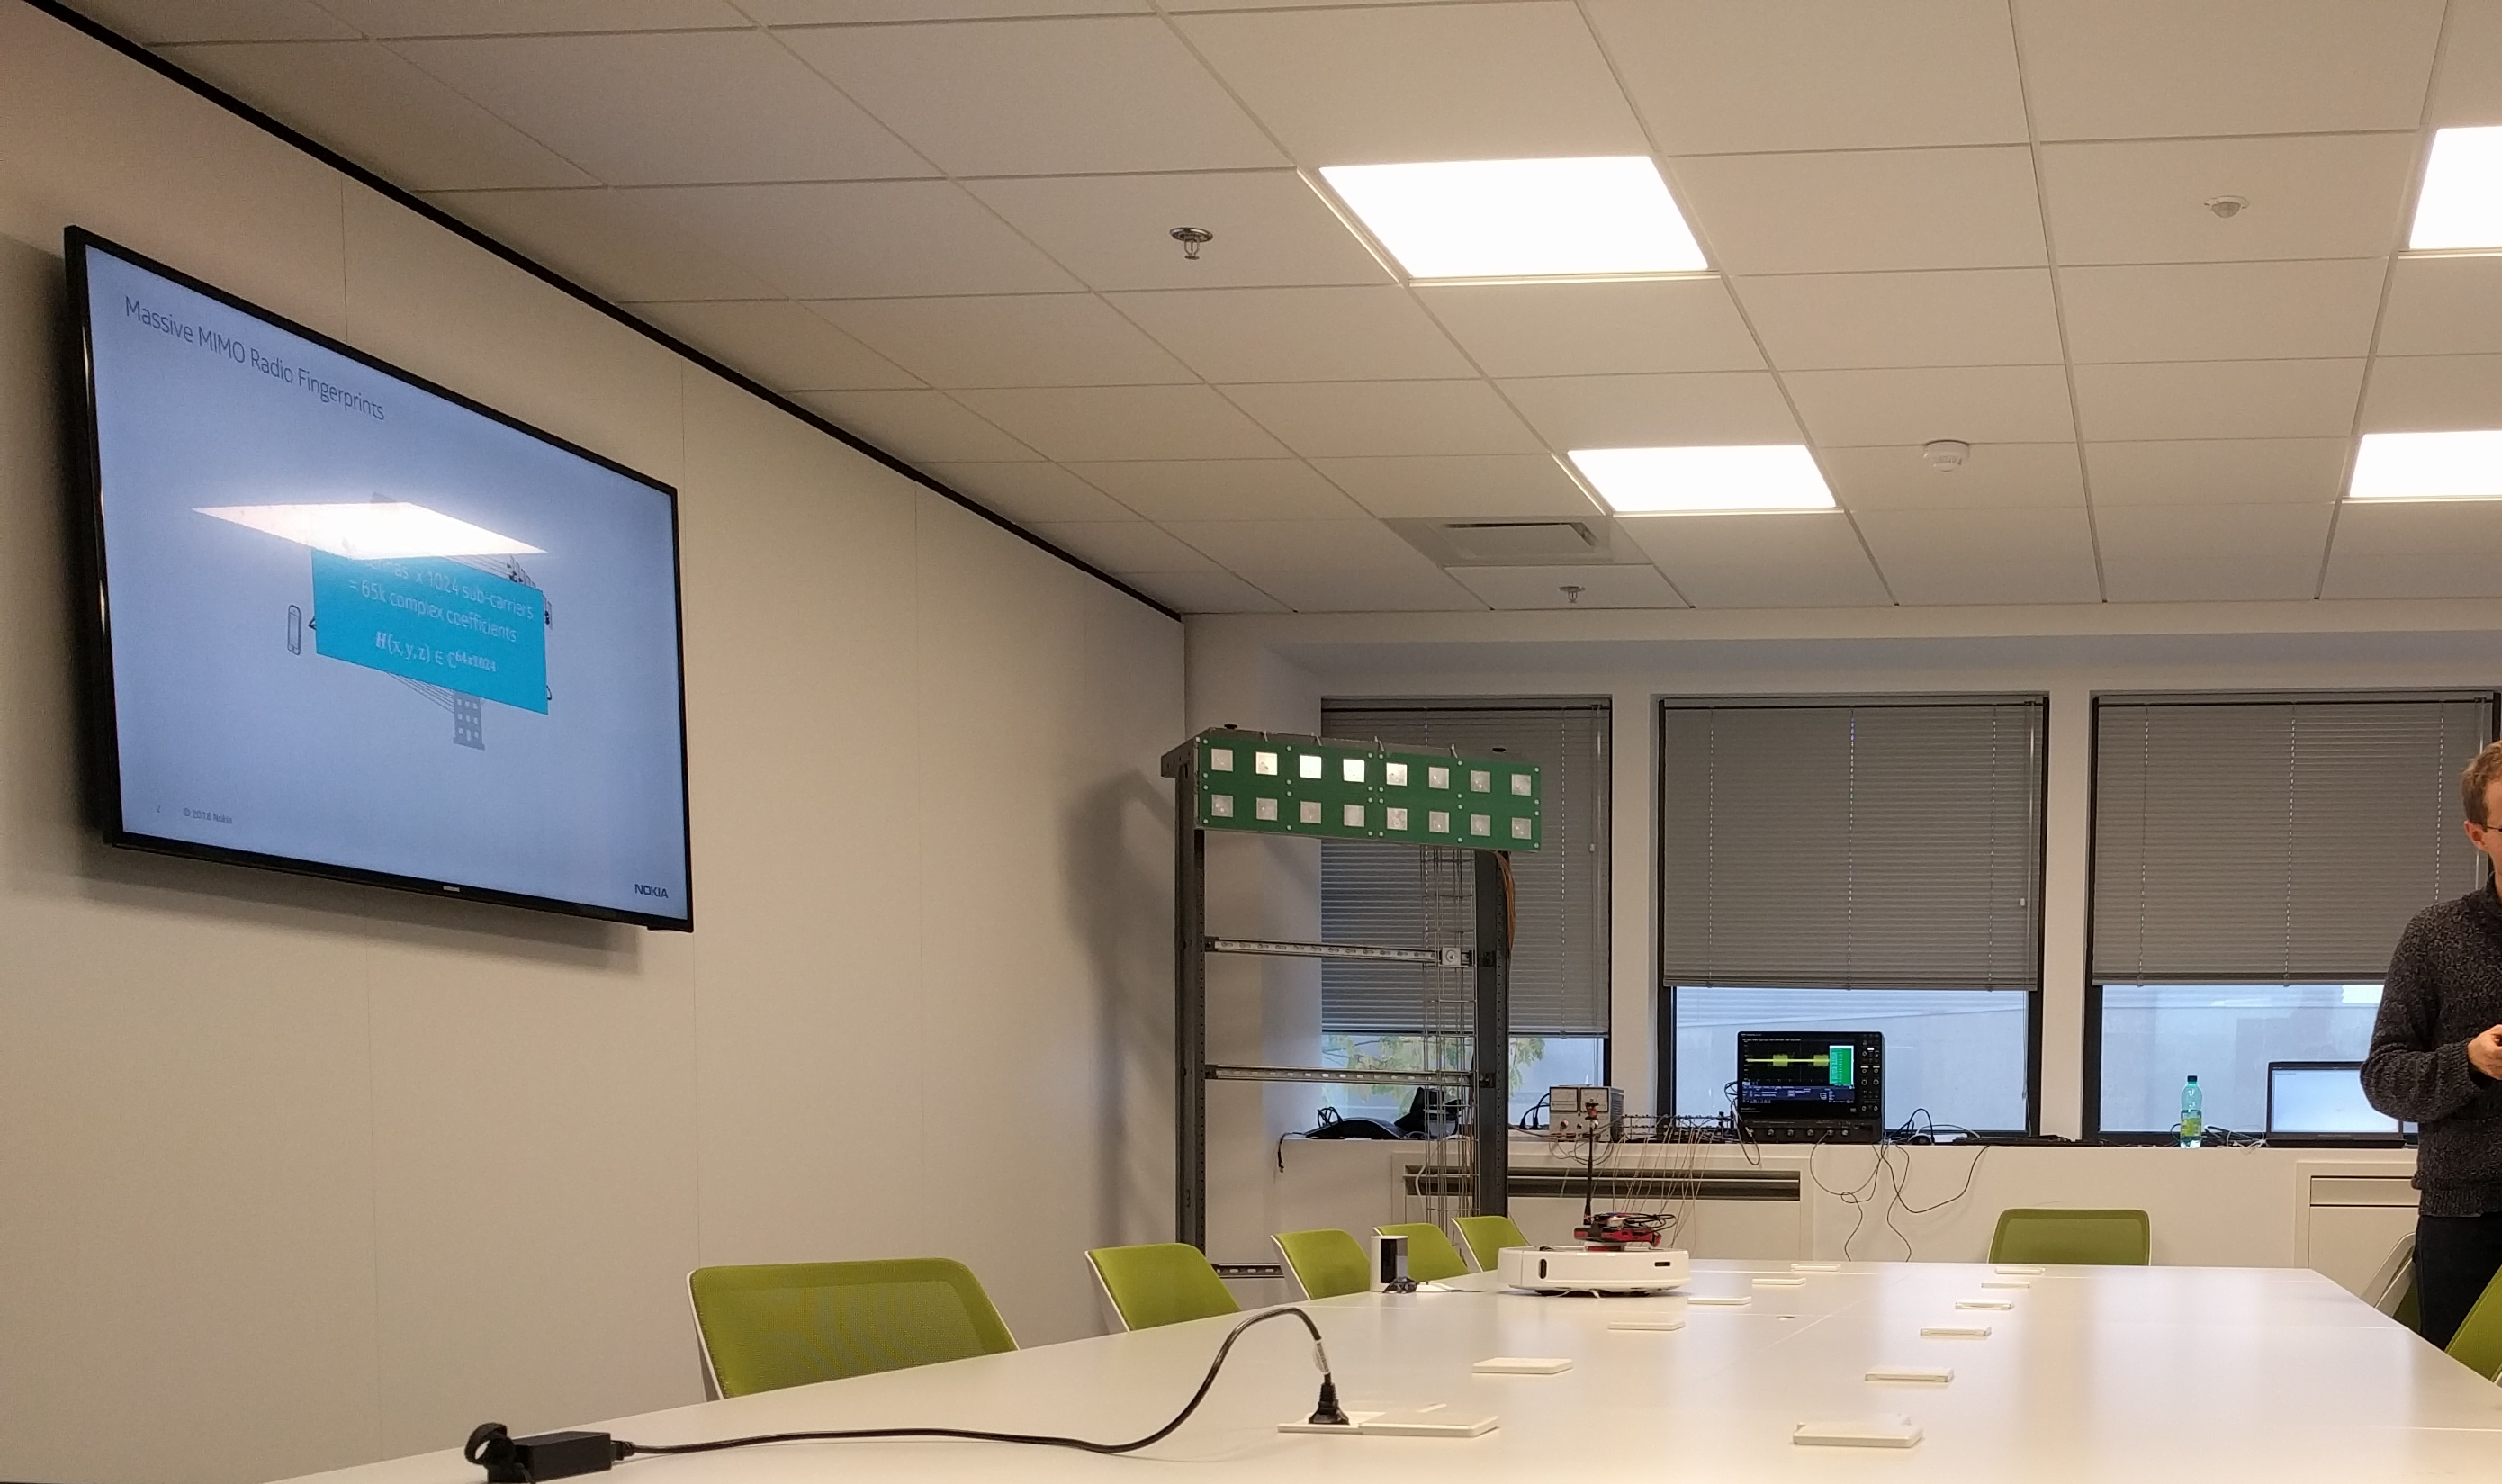
\includegraphics[width=0.5\textwidth]{ParisEnvironment}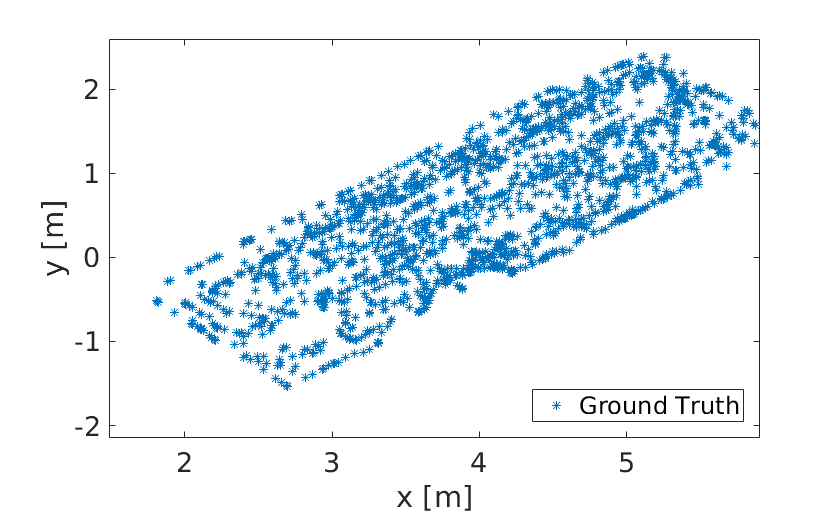
\includegraphics[width=0.5\textwidth]{IndoorDataset}
The left Fig. shows a picture of the measurement scenario. On the right hand the ``Ground Truth'' Points created by a Tachymeter with an accuracy below 1cm is shown.
\vspace{4ex}


~

The dataset is provided in three different formats (.mat, h5, and pickle), and    available via the following links: \newline
  MAT:    \url{https://drive.google.com/open?id=11IGqnn9k8vjkgfMG4G0-AYTgIA5CoDMW} \newline
  HDF;    \url{https://drive.google.com/open?id=11qtImrA8Y12L_2RncRC12GXKo0pdrYhT} \newline
  PICKLE: \url{https://drive.google.com/open?id=1HNXjmyMZe6D828oYuhEQqmW5jwf4wy_I} \newline

~

The dataset contains three main files: the channels, the positions, and the SNRs. The channel variable is called ``h\_Estimated'' with the dimension of [Number of measured Points x Number of antennas (16) x Number of used subcarriers (924)]. The position is given in the ``r\_Position'' variable with dimensions of the number of points  and there coordinates [x,y,z] (in this order). The last variable contains the SNR of each antenna at each point resulting in the dimensions 
of [Number of measured Points x Number of antennas].

~


To get started with the competition, find further details in the README and the basic Jupyter Notebook provided in the following link:\newline
\url{https://github.com/MaximilianArnold/CTW2019-PositioningCompetition}



%~

%To get an idea of the SNR of the data, the following figure shows a CDF plot for all antennas stacked of the SNR. Therefore the signal quality is in a quite reasonable range.

%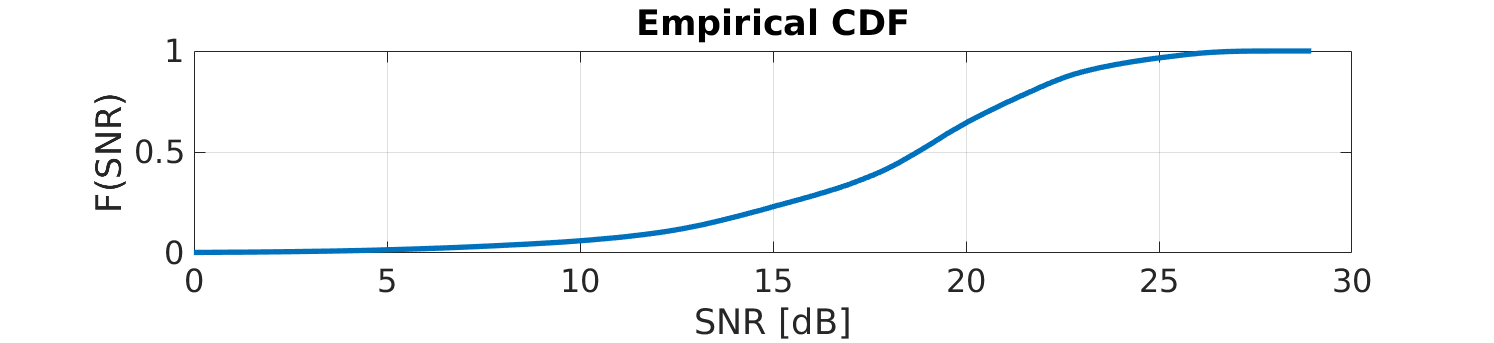
\includegraphics[width=1\textwidth]{ChannelQuality}


%~

\section{Reference}%
[1] Maximilian Arnold, Jakob Hoydis, and Stephan ten Brink,  ``Novel Massive MIMO Channel Sounding Data applied to Deep Learning-based Indoor Positioning'', Submitted to SCC2019.

[Online]. Available: arXiv:https://arxiv.org/abs/1810.04126

\section{Contact}

\begin{itemize}
\item Questions about the dataset: \\
-- Maximilian Arnold, \texttt{maximilian.arnold@inue.uni-stuttgart.de} \\
-- Prof. Stephan ten Brink, \texttt{
	tenbrink@inue.uni-stuttgart.de} \\

\item General questions about the CTW competition: \\
-- Prof. Erik G. Larsson, \texttt{erik.g.larsson@liu.se} (2019 IEEE CTW technical co-chair) \\
-- Prof. Urbashi Mitra, \texttt{ubli@usc.edu} (2019 IEEE CTW technical co-chair) 

\end{itemize}

\vspace{10ex}

%
\includegraphics[width=1\textwidth]{Comsoc}

\end{document}
